% Comment with '%' to remove all comments at once
\def \Commentaires{}

\documentclass[svgnames,table,runningheads]{llncs}
\usepackage[english]{babel}
\usepackage[T1]{fontenc} 
\usepackage[utf8]{inputenc}
\usepackage{url}
\usepackage{xspace}
\usepackage{lmodern} % for textsc
\usepackage{subcaption}

\usepackage{graphicx}
\usepackage{booktabs}
\usepackage{amsmath,amssymb}
\usepackage{microtype}
\usepackage{colortbl}
\usepackage{tikz}
\usetikzlibrary{arrows.meta, positioning, fit, shapes.geometric, math, calc}
\usepackage[linesnumbered,boxed,ruled,vlined]{algorithm2e}
\usepackage{pgfplots}

\usepackage{authblk} % for authors affiliation
\usepackage{enumitem} % for enumeration without indentation
\usepackage{wrapfig}

\usepackage{hyperref}
\hypersetup{
  colorlinks   = true, %Colours links instead of ugly boxes
  urlcolor     = blue, %Colour for external hyperlinks
  linkcolor    = blue, %Colour of internal links
  citecolor   = blue, %Colour of citations
  breaklinks = true %use \href{url}{\nolinkurl{display URL}} for breakable long URLs
}

\usepackage{multirow}
\usepackage{xcolor}

\ifdefined\Commentaires
\newcommand{\gn}[1]{\noindent{\color{orange}GN: #1}\xspace}
\newcommand{\fr}[1]{\noindent{\color{red}FR: #1}\xspace}
\else
\newcommand{\gn}[1]{}
\newcommand{\fr}[1]{}
\fi

\renewcommand{\thealgocf}{}
\pgfplotsset{
  compat=newest,
  xlabel near ticks,
  ylabel near ticks
}
% ----- Colors -----
\definecolor{myblue}{RGB}{31,95,255}
\definecolor{mygreen}{RGB}{47,214,58}
\definecolor{myred}{RGB}{255,42,31}

% ----- Styles -----
\tikzset{
  box/.style={line width=1.6pt, line join=miter}, % all straight lines
  num/.style={font=\bfseries\Large}
}

% Grid size (in unit cells): 10 wide x 5 tall. Every box is 2x1.
\newcommand{\GW}{10}
\newcommand{\GH}{5}

\pgfkeys{
  mybox/.is family,
  mybox,
  x/.initial=0,
  y/.initial=0,
  height/.initial=\GH,
  color/.initial=myblue,
  text/.initial={}, 
}

\newcommand\myboxset[1]{\pgfkeys{mybox,#1}}
\newcommand\myvbox[1][]{
  \myboxset{#1,
    x/.get=\boxx,
    y/.get=\boxy,
    height/.get=\gridheight,
    color/.get=\boxcolor,
    text/.get=\boxtext
  }

  \draw[box,\boxcolor] (\boxx+0.1,\gridheight-\boxy-0.1) rectangle (\boxx+0.9,\gridheight-\boxy-1.9);
  \node[num,\boxcolor] at (\boxx+0.5,\gridheight-\boxy-1) {\boxtext};
}
\newcommand\myhbox[1][]{
  \myboxset{#1,
    x/.get=\boxx,
    y/.get=\boxy,
    height/.get=\gridheight,
    color/.get=\boxcolor,
    text/.get=\boxtext
  }

  \draw[box,\boxcolor] (\boxx+0.1,\gridheight-\boxy-0.1) rectangle (\boxx+1.9,\gridheight-\boxy-0.9);
  \node[num,\boxcolor] at (\boxx+1,\gridheight-\boxy-0.5) {\boxtext};
}

\title{Random Edmonds--Karp for Generating Valid Solutions to Sabrina's Game}
\titlerunning{Random Edmonds--Karp for Sabrina's Game}

% \author{Anonymous Author(s)}
% \authorrunning{Anonymous Author(s)}
% \institute{Anonymous institute(s)\\\email{anonymous@example.org}}

\author{Florian Richoux\inst{1}\orcidID{0000-0003-4693-379X} \and
Daan van den Berg\inst{2}\orcidID{0000-0001-5060-3342}}
%
\authorrunning{F. Richoux and D. van den Berg}
\institute{AIST, Japan\\
\email{florian.richoux@aist.go.jp}\\
\and
Vrije Universiteit Amsterdam, The Netherlands\\
\email{d.van.den.berg@vu.nl}
}

\begin{document}
\maketitle

\begin{abstract}
Sabrina's Game asks for a domino tiling of a rectangular grid that minimizes a cost associated with adjacent paired cells. Before optimization, evolutionary methods require a mechanism for generating feasible tilings. We study the satisfaction version of the problem and ask whether valid solutions can be sampled uniformly at random in polynomial time. We model a tiling as a perfect matching in the bipartite grid graph and introduce \emph{Random Edmonds--Karp}, a randomized variant of the Edmonds--Karp algorithm in which the adjacency lists explored by each breadth-first search are shuffled. The procedure always returns a valid tiling on the considered even square grids and inherits polynomial worst-case time from Edmonds--Karp. Experiments show that it does not sample uniformly, but produces substantially varied tilings at low computational cost. Over $10^6$ runs for every square size from $4\times4$ to $20\times20$, the mean runtime grows from $17.33\,\mu$s to $11.89\,$ms, while measured memory consumption grows from $7904$ to $9884$ kB. These results position Random Edmonds--Karp as a practical initializer for evolutionary search, while leaving exact or approximate uniform sampling as an open direction.
\keywords{Domino tiling \and Random generation \and Edmonds--Karp \and Perfect matching \and Evolutionary computation}
\end{abstract}

\section{Introduction}
Population-based evolutionary algorithms need a sufficiently diverse initial population. For highly constrained combinatorial problems, generating feasible individuals can itself be a major obstacle. Sabrina's Game is a deliberately simple example: a rectangular array of values must be partitioned into horizontal or vertical dominoes, and the optimization version minimizes the sum of the absolute differences between the two values covered by each domino. Its satisfaction version ignores cell values and asks only for a valid domino tiling.

The initial question of this study is whether feasible tilings can be generated both uniformly and in polynomial time. Uniformity is attractive because it avoids an algorithm-dependent bias in the initial population. However, practical evolutionary search may not require perfect uniformity: a fast generator that reliably returns valid and varied solutions can already be useful.

A domino tiling is equivalent to a perfect matching in a grid graph. Since the square grid graph is bipartite, feasibility can be reduced to maximum flow. This observation gives a deterministic polynomial-time decision and construction procedure. Yet a fixed search order tends to return highly structured matchings. We therefore randomize the order in which breadth-first search explores vertices within Edmonds--Karp. The resulting method, called Random Edmonds--Karp (REK), preserves feasibility and polynomial-time termination, although it does not induce the uniform distribution over perfect matchings.

Our contributions are:
\begin{itemize}
  \item a flow formulation of the satisfaction version of Sabrina's Game;
  \item Random Edmonds--Karp, a simple randomized polynomial-time generator of valid tilings;
  \item an empirical rejection of exact uniformity on the $4\times4$ instance using $10^6$ samples; and
  \item a scaling study of iterations, runtime, and memory on all even square grids from $4\times4$ to $20\times20$, with $10^6$ runs per size.
\end{itemize}

\section{Sabrina's Game and Domino Tilings}
Let $R_{m,n}=\{1,\ldots,m\}\times\{1,\ldots,n\}$ be an $m\times n$ rectangular grid. A domino is an unordered pair of adjacent cells. A feasible solution is a set $D$ of dominoes such that every cell occurs in exactly one domino. Therefore, $mn$ must be even.

For the optimization version, each cell $u$ has a value $a_u$, and the objective is
\begin{equation}
  \min_{D} \sum_{\{u,v\}\in D}|a_u-a_v|.
\end{equation}

\fr{Cite Daan's work}

The present work considers only satisfaction: finding any feasible $D$. This is precisely the classical domino-tiling problem, equivalently a perfect matching of the grid graph~\cite{fusy2016random}.

\begin{figure}
  \begin{tikzpicture}[scale=1.0]
    \draw[black,line width=0.4pt,step=1] (0,0) grid (4,4);
    \draw[black,line width=1.6pt] (0,0) rectangle (4,4);
    
    \draw[box,fill=myblue,myblue] (0+0.1,4-0-0.1) rectangle (0+1.9,4-0-0.9);
    \draw[box,fill=myblue,myblue] (2+0.1,4-0-0.1) rectangle (2+1.9,4-0-0.9);

    \draw[box,fill=myblue,myblue] (0+0.1,4-1-0.1) rectangle (0+0.9,4-1-1.9);
    \draw[box,fill=myblue,myblue] (1+0.1,4-1-0.1) rectangle (1+1.9,4-1-0.9);
    \draw[box,fill=myblue,myblue] (3+0.1,4-1-0.1) rectangle (3+0.9,4-1-1.9);

    \draw[box,fill=myblue,myblue] (1+0.1,4-2-0.1) rectangle (1+1.9,4-2-0.9);

    \draw[box,fill=myblue,myblue] (0+0.1,4-3-0.1) rectangle (0+1.9,4-3-0.9);
    \draw[box,fill=myblue,myblue] (2+0.1,4-3-0.1) rectangle (2+1.9,4-3-0.9);
  \end{tikzpicture}
  \begin{tikzpicture}[scale=1.0]
    \draw[black,line width=0.4pt,step=1] (0,0) grid (4,4);
    \draw[black,line width=1.6pt] (0,0) rectangle (4,4);
    
    \draw[box,fill=myred,,line width=0.6pt] (-1+0.1,4-0-0.1) rectangle (-1+1.9,4-0-0.9);
    \draw[box,fill=myblue,myblue] (2+0.1,4-0-0.1) rectangle (2+1.9,4-0-0.9);

    \draw[box,fill=myblue,myblue] (0+0.1,4-1-0.1) rectangle (0+0.9,4-1-1.9);
    \draw[box,fill=myblue,myblue] (1+0.1,4-1-0.1) rectangle (1+1.9,4-1-0.9);
    \draw[box,fill=myred,line width=0.6pt] (3+0.1,4-2-0.1) rectangle (3+0.9,4-2-1.9);

    \draw[box,fill=myblue,myblue] (1+0.1,4-2-0.1) rectangle (1+1.9,4-2-0.9);

    \draw[box,fill=myblue,myblue] (0+0.1,4-3-0.1) rectangle (0+1.9,4-3-0.9);
    \draw[box,fill=myred,,line width=0.6pt] (2+0.1,4-3-0.1) rectangle (2+1.9,4-3-0.9);

    \node[num,myred] at (1.5,3.5) {X};
    \node[num,myred] at (3.5,2.5) {X};
  \end{tikzpicture}
  \caption{Left: An expected perfect tiling. Right: An invalid solution, with two cells not covered by any tile, a tile going outside the frame, and two overlapping tiles}\label{fig:tiling}
\end{figure}

\fr{Chessboard and bipartite graph figures}

\begin{figure}
  \centering
  \begin{tikzpicture}[scale=1.0]
    \draw[lightgray,line width=0.4pt,step=1] (0,0) grid (4,4);
    \draw[black,line width=1.6pt] (0,0) rectangle (4,4);
    
    \draw[fill=black,black] (0,0) rectangle (1,1);
    \draw[fill=black,black] (2,0) rectangle (3,1);
    \draw[fill=black,black] (1,1) rectangle (2,2);
    \draw[fill=black,black] (3,1) rectangle (4,2);
    \draw[fill=black,black] (0,2) rectangle (1,3);
    \draw[fill=black,black] (2,2) rectangle (3,3);
    \draw[fill=black,black] (1,3) rectangle (2,4);
    \draw[fill=black,black] (3,3) rectangle (4,4);
  \end{tikzpicture}
  \begin{tikzpicture}[scale=1.0]
    \draw[lightgray,line width=0.4pt,step=1] (0,0) grid (4,4);
    \draw[black,line width=1.6pt] (0,0) rectangle (4,4);
    
    \draw[black,line width=1pt] (0.5,0.5) -- (3.5,0.5);
    \draw[black,line width=1pt] (0.5,1.5) -- (3.5,1.5);
    \draw[black,line width=1pt] (0.5,2.5) -- (3.5,2.5);
    \draw[black,line width=1pt] (0.5,3.5) -- (3.5,3.5);
    \draw[black,line width=1pt] (0.5,0.5) -- (0.5,3.5);
    \draw[black,line width=1pt] (1.5,0.5) -- (1.5,3.5);
    \draw[black,line width=1pt] (2.5,0.5) -- (2.5,3.5);
    \draw[black,line width=1pt] (3.5,0.5) -- (3.5,3.5);

    \draw[black,fill=black] (0.5,0.5) circle (0.25);
    \draw[black,fill=white] (0.5,1.5) circle (0.25);
    \draw[black,fill=black] (0.5,2.5) circle (0.25);
    \draw[black,fill=white] (0.5,3.5) circle (0.25);

    \draw[black,fill=white] (1.5,0.5) circle (0.25);
    \draw[black,fill=black] (1.5,1.5) circle (0.25);
    \draw[black,fill=white] (1.5,2.5) circle (0.25);
    \draw[black,fill=black] (1.5,3.5) circle (0.25);

    \draw[black,fill=black] (2.5,0.5) circle (0.25);
    \draw[black,fill=white] (2.5,1.5) circle (0.25);
    \draw[black,fill=black] (2.5,2.5) circle (0.25);
    \draw[black,fill=white] (2.5,3.5) circle (0.25);

    \draw[black,fill=white] (3.5,0.5) circle (0.25);
    \draw[black,fill=black] (3.5,1.5) circle (0.25);
    \draw[black,fill=white] (3.5,2.5) circle (0.25);
    \draw[black,fill=black] (3.5,3.5) circle (0.25);
  \end{tikzpicture}
  \begin{tikzpicture}[scale=1.0]
    \draw[black,line width=1pt] (0,0) -- (0,2);
    \draw[black,line width=1pt] (0,0) -- (1,2);
    \draw[black,line width=1pt] (0,0) -- (2,2);

    \draw[black,line width=1pt] (1,0) -- (1,2);
    \draw[black,line width=1pt] (1,0) -- (3,2);

    \draw[black,line width=1pt] (2,0) -- (0,2);
    \draw[black,line width=1pt] (2,0) -- (2,2);
    \draw[black,line width=1pt] (2,0) -- (4,2);

    \draw[black,line width=1pt] (3,0) -- (1,2);
    \draw[black,line width=1pt] (3,0) -- (2,2);
    \draw[black,line width=1pt] (3,0) -- (3,2);
    \draw[black,line width=1pt] (3,0) -- (5,2);

    \draw[black,line width=1pt] (4,0) -- (2,2);
    \draw[black,line width=1pt] (4,0) -- (4,2);
    \draw[black,line width=1pt] (4,0) -- (5,2);
    \draw[black,line width=1pt] (4,0) -- (6,2);

    \draw[black,line width=1pt] (5,0) -- (3,2);
    \draw[black,line width=1pt] (5,0) -- (5,2);
    \draw[black,line width=1pt] (5,0) -- (7,2);

    \draw[black,line width=1pt] (6,0) -- (4,2);
    \draw[black,line width=1pt] (6,0) -- (6,2);

    \draw[black,line width=1pt] (7,0) -- (5,2);
    \draw[black,line width=1pt] (7,0) -- (6,2);
    \draw[black,line width=1pt] (7,0) -- (7,2);

    \draw[black,fill=white] (0,2) circle (0.25);
    \draw[black,fill=white] (1,2) circle (0.25);
    \draw[black,fill=white] (2,2) circle (0.25);
    \draw[black,fill=white] (3,2) circle (0.25);
    \draw[black,fill=white] (4,2) circle (0.25);
    \draw[black,fill=white] (5,2) circle (0.25);
    \draw[black,fill=white] (6,2) circle (0.25);
    \draw[black,fill=white] (7,2) circle (0.25);

    \draw[black,fill=black] (0,0) circle (0.25);
    \draw[black,fill=black] (1,0) circle (0.25);
    \draw[black,fill=black] (2,0) circle (0.25);
    \draw[black,fill=black] (3,0) circle (0.25);
    \draw[black,fill=black] (4,0) circle (0.25);
    \draw[black,fill=black] (5,0) circle (0.25);
    \draw[black,fill=black] (6,0) circle (0.25);
    \draw[black,fill=black] (7,0) circle (0.25);  
  \end{tikzpicture}
  \caption{Grid as a Chessboard}\label{fig:chessboard}
\end{figure}


Color the grid as a chessboard and let $B$ and $W$ denote the black and white cells. Every adjacency joins one cell in $B$ to one in $W$, so the grid graph $G=(B\cup W,E)$ is bipartite. Construct a flow network by adding a source $s$, a sink $t$, unit-capacity arcs from $s$ to every vertex in $B$, unit-capacity arcs corresponding to grid adjacencies from $B$ to $W$, and unit-capacity arcs from every vertex in $W$ to $t$. An integral flow of value $mn/2$ is equivalent to a perfect matching and thus to a valid tiling.

\section{Random Edmonds--Karp}
Edmonds--Karp repeatedly finds a shortest augmenting path in the residual network by breadth-first search (BFS). Its generic worst-case complexity is $O(|V|\cdot |E|^2)$~\cite{edmondskarp1972}. The randomization used here changes only tie-breaking among nodes at the same BFS depth. Consequently, every selected augmenting path remains shortest, and the standard complexity result still applies.

% \begin{algorithm}[t]
% \caption{Random Edmonds--Karp for domino tiling}\label{alg:rek}
% \begin{algorithmic}[1]
% \Require Flow network $N=(V,A)$ constructed from an even grid
% \Ensure A perfect matching, or failure if none exists
% \State $f\gets 0$
% \While{$t$ is reachable from $s$ in the residual network $N_f$}
%   \ForAll{$u\in V$}
%     \State randomly shuffle the residual outgoing arcs of $u$
%   \EndFor
%   \State $P\gets$ a shortest $s$--$t$ path returned by BFS
%   \State augment one unit of flow along $P$
% \EndWhile
% \If{$|f|=mn/2$}
%   \State \Return the dominoes induced by the $B$--$W$ arcs carrying flow
% \Else
%   \State \Return failure
% \EndIf
% \end{algorithmic}
% \end{algorithm}

% \begin{algorithm}
%   \DontPrintSemicolon
%   $flow \gets \emptyset$\;
%   \While{$\text{a simple path from S to T exists}$}{
%     \ForEach{$edge\ (x,y) \text{ in the path}$}{
%       \If{$(x,y) \text{ is an edge in the original graph}$}{
%         $flow \gets flow \cup (x,y)$\;
%       }
%       \Else{
%         $flow \gets flow \setminus (x,y)$\;
%       }
%       Flip edge $(x,y)$\;
%     }          
%   }
%   \Return $flow$\;
%   \caption{Ford-Fulkerson}\label{alg:rek} 
% \end{algorithm}

\begin{algorithm}
  \DontPrintSemicolon
  $flow \gets \emptyset$\;
  \While{$\text{source } S \text{ has a child}$}{
    $path \gets S$\;
    $path \gets make\_path(path)$\;
    \For{$i\text{ from 0 to path.length-1}$}{
      \If{$flow.contains(edge(path[i+1], path[i]))$}{
        $flow.remove(edge(path[i+1], path[i]))$\;
      }
      $flow.add(edge(path[i], path[i+1]))$\;
      Flip $edge(path[i], path[i+1])$\;
    }
  }
  \Return $flow$\;
  \caption{Random Edmonds--Karp}\label{alg:rek} 
\end{algorithm}

\begin{algorithm}
  \DontPrintSemicolon
  \KwIn{A path containing source $S$ only}
  \KwOut{A random path from source $S$ to sink $T$}

  $queue \gets emptyset$\;
  $queue.push(S)$\;
  \While{$queue~!=~\emptyset$}{
    $current \gets queue.pop()$\;
    \If{$current~==~T$}{
      Stop\;
    }
    \Else{
      Shuffle($current.children$)\;
      \ForEach{$child \text{ in } current.children$}{
        \If{$child \text{ not visited}$}{
          $queue.push(child)$\;
          Mark $child$ as visited\;
        }
      }
    }
  }
  $stack \gets \emptyset$\;
  \While{$current~!=~S$}{
    $stack.push(current)$\;
    $current \gets current.parent$\;
  }
  \While{$stack~!=~\emptyset$}{
    $current \gets stack.pop()$\;
    $path \gets concat(path, current)$\;
  }
  \Return $path$\;
  \caption{make\_path}\label{alg:path} 
\end{algorithm}

\subsection{Correctness and complexity}

\begin{proposition}
Algorithm~\ref{alg:rek} returns a maximal flow of $mn/2$.
\end{proposition}
\begin{proof}
Each iteration of Algorithm~\ref{alg:rek} is adding one edge into the flow, even if some edges are removed. Indeed, removing an edge from the flow means that the path contains a flipped edge from a black node to a white node. However, the path necessarily contains a ``white-to-black'' edge for each ``black-to-white'' edge, to reach the sink \(t\). This implies that each edge removal from the flow is compensated by the addition of another edge in the flow. Thus, for \(k\) ``black-to-white'' edges in the path, the later contains exactly \(k+1\) ``white-to-black'' edges.

All capacities between white and black nodes are equal to 1, so each flow augmentation will increase by 1. Algorithm~\ref{alg:rek} selects a total of $mn/2$ paths (since there are $mn/2$ white nodes, thus $mn/2$ arcs from \(s\) to a white node), which implies $mn/2$ flow augmentations. The algorithm returns a maximal flow of $mn/2$.
\end{proof}

\fr{Add a Lemma showing that no edges in the flow contain twice the same node. Thus flow of \(mn/2 \Rightarrow\) valid tiling}

\begin{proposition}\label{prop:complexity}
Random Edmonds--Karp terminates in polynomial time.
\end{proposition}
\begin{proof}
At each iteration, Algorithm~\ref{alg:rek} consumes one edge from \(s\) to a white node, and reciprocaly one edge from a black node to \(t\), so it necessarily terminates after \(mn/2\) iterations, since no paths from \(s\) to \(t\) remain once all ``s-to-white'' and ``black-to-t'' edges have been flipped.

Finding a path is done with Breadth-First Search, which is in \(O(|V|+|E|)\), and shuffling the children of a node is done in constant time, since no nodes has more than 4 children. Therefore the standard Edmonds--Karp bound $O(|V|\cdot |E|^2)$ applies. For an $n\times m$ grid, $|V|=mn+2$ and $|E|=\Theta(mn)$ in the flow network. Therefore, Algorithm~\ref{alg:rek} runs in polynomial-time in the problem instance size.
\end{proof}

\subsection{Why the distribution is not uniform}
Random tie-breaking does not assign equal probability to all perfect matchings. A final matching can be reached through many sequences of shortest augmenting paths, and different matchings need not have the same number or probability mass of such histories. On the $4\times4$ grid, which has 36 tilings, the frequencies observed over $10^6$ independent runs reject the uniform null hypothesis under Pearson's chi-squared test at the 5\% significance level. Thus REK should be described as a randomized feasible-solution generator, not as a uniform sampler.

\fr{Figures from my slides}

\begin{figure}
  \begin{tikzpicture}[scale=0.75]
    \begin{axis}[
      width=16cm, height=9cm,
      ybar,                          % one bar per data point
      bar width=8pt,
      xlabel={Solution},
      ylabel={Frequency},
      xmin=0.5, xmax=36.5,
      ymin=0,   ymax=61000,
      xtick={1,2,...,36},
      xticklabel style={font=\footnotesize},
      yticklabel style={/pgf/number format/1000 sep={\,}},
      ymajorgrids=true,
      grid style={gray!30},
      tick align=outside,
      enlarge x limits=0.02,
      fill=blue!60, draw=black,
      ]
      % x = value (1..36), y = frequency
      \addplot+[ybar] coordinates {
        (1,19267)  (2,20955)  (3,25702)  (4,20188) (5,21353)  (6,33822)
        (7,32129)  (8,20204)  (9,21027)  (10,29825) (11,21873) (12,20954)
        (13,59965) (14,25656) (15,31980) (16,31251) (17,30031) (18,34359)
        (19,34039) (20,30023) (21,20886) (22,21868) (23,31966) (24,20979)
        (25,20428) (26,31167) (27,31779)  (28,25745) (29,59932) (30,30067)
        (31,25474) (32,20899) (33,20218) (34,33744) (35,20896)  (36,19349)
      };
    \end{axis}
  \end{tikzpicture}
  \caption{Solution distribution over 1,000,000 runs on a \(4times4\) grid}\label{fig:notuniform}
\end{figure}

\begin{figure}
  \begin{tikzpicture}[scale=1]
    \draw[lightgray,line width=0.4pt,step=1] (0,0) grid (4,4);
    \draw[black,line width=1.6pt] (0,0) rectangle (4,4);
    
    \myvbox[x=0,y=0,height=4,color=myblue]
    \myhbox[x=1,y=0,height=4,color=myblue]
    \myvbox[x=3,y=0,height=4,color=myblue]
    \myvbox[x=0,y=2,height=4,color=myblue]
    \myvbox[x=1,y=1,height=4,color=myblue]
    \myvbox[x=2,y=1,height=4,color=myblue]
    \myhbox[x=1,y=3,height=4,color=myblue]
    \myvbox[x=3,y=2,height=4,color=myblue]
  \end{tikzpicture}
  \begin{tikzpicture}[scale=1]
    \draw[lightgray,line width=0.4pt,step=1] (0,0) grid (4,4);
    \draw[black,line width=1.6pt] (0,0) rectangle (4,4);
    
    \myhbox[x=0,y=0,height=4,color=myblue]
    \myhbox[x=2,y=0,height=4,color=myblue]
    \myvbox[x=0,y=1,height=4,color=myblue]
    \myhbox[x=1,y=1,height=4,color=myblue]
    \myhbox[x=1,y=2,height=4,color=myblue]
    \myvbox[x=3,y=1,height=4,color=myblue]
    \myhbox[x=0,y=3,height=4,color=myblue]
    \myhbox[x=2,y=3,height=4,color=myblue]
  \end{tikzpicture}
  \caption{The two most frequent solutions are very symmetrical}\label{fig:sym}
\end{figure}

\fr{About the Pearson test, give the degrees of freedom, $p$-value, etc.}

\section{Experimental Methodology}
We evaluated square grids of side $n\in\{4,6,8,10,12,14,16,18,20\}$. Each configuration was executed $10^6$ times. We recorded the mean runtime in microseconds, and the program memory in kilobytes. All experiments have been done on GNU/Linux CachyOS over a machine with a Core i9 9900 CPU and 32 GB of RAM. The C++ code has been compiled with g++ v16.2.1, with the -O3 optimization flag. The source code, the experimental setup and the result summaries can be found at URL
%\href{https://anonymous.4open.science/r/...}{anonymous.4open.science/r/...}.
% \href{https://github.com/richoux/Sabrina-s-Game/tree/...}{github.com/richoux/Sabrina-s-Game/tree/...}.

The number of while-loop interations is deterministic in these experiments: all grids are tileable and every augmentation carries one unit, hence $n^2/2$ iterations are required. Runtime and memory values are aggregate measurements supplied by the implementation.

\section{Results}
\begin{table}[t]
\centering
\caption{Performance over $10^6$ runs per square grid size.}\label{tab:results}
\begin{tabular}{rrrr}
\toprule
Grid & Iterations & Mean runtime ($\mu$s) & Memory (kB)\\
\midrule
$4\times4$   & 8   & 17.33   & 7904\\
$6\times6$   & 18  & 94.38   & 8036\\
$8\times8$   & 32  & 285.17  & 8168\\
$10\times10$ & 50  & 710.46  & 8300\\
$12\times12$ & 72  & 1475.76 & 8564\\
$14\times14$ & 98  & 2760.32 & 8828\\
$16\times16$ & 128 & 4736.52 & 9120\\
$18\times18$ & 162 & 7555.95 & 9484\\
$20\times20$ & 200 & 11898.37 & 9884\\
\bottomrule
\end{tabular}
\end{table}

\begin{figure}[t]
\centering
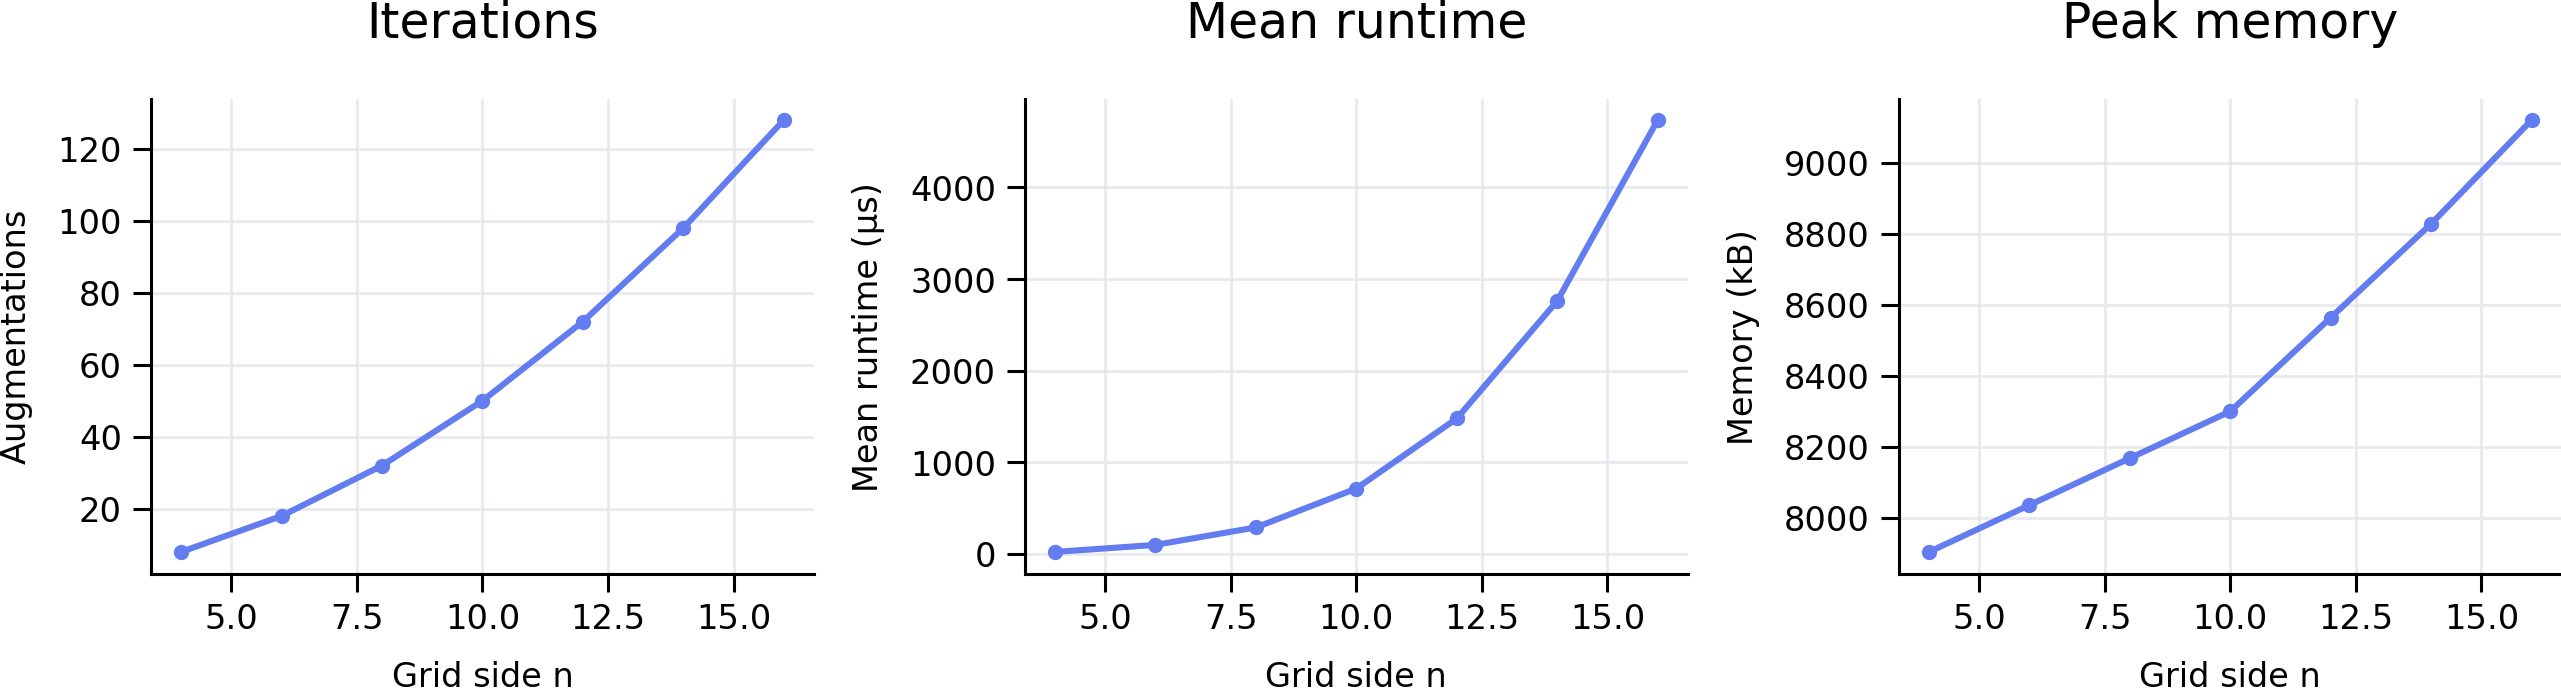
\includegraphics[width=\textwidth]{figs/rek_scaling}
\caption{Number of while-loop iterations, mean runtime, and memory consumption as the square grid side increases.}\label{fig:scaling}
\end{figure}

The mean runtime remains below 12ms even for the $20\times20$ grid. A descriptive power-law regression on the seven means gives approximately $T(n)=a n^{p}$ with $p=4.02$. This is not a complexity proof, but it suggests quartic growth over the measured range, substantially below the conservative generic bound given in the proof of Proposition~\ref{prop:complexity}. Runtime increases by a factor of about 686 between $n=4$ and $n=20$, while the number of cells increases by a factor of 25.

Measured memory increases by 1980kB, or approximately 25\%, across the tested range. A linear fit against the grid side starting from \(10\times10\) gives about 156kB per additional row/column over this narrow interval. Because the measurement includes a large fixed program baseline, these values do not directly establish an asymptotic space complexity.

\section{Discussion}
The central result is practical rather than distributional. REK does not solve the initial uniform-sampling question, but it combines three useful properties: it always constructs a feasible tiling, it has a polynomial worst-case guarantee, and randomized BFS tie-breaking yields visibly different solutions. This makes it suitable for initializing evolutionary or other population-based methods without repair or rejection sampling.

The non-uniformity result requires careful interpretation. Rejecting exact uniformity does not show that the distribution is unusably concentrated. % For evolutionary computation, more relevant diagnostics include entropy, effective support size, pairwise Hamming distance between matchings, edge-inclusion marginals, and downstream optimization performance. These should be added in the next experimental revision.
Exact uniform samplers exist for important special regions, such as domino shuffling for Aztec diamonds, while more general approaches often use Markov chains~\cite{nordenstam2008shuffling,fusy2016random}. Their objectives and computational trade-offs differ from the deliberately simple REK procedure.
\fr{Not really sure about this -> to check}

Several limitations remain. First, the present scaling study covers only small squares. Second, mean runtime alone does not characterize variability; standard deviation and quantiles should be reported. 

\section{Conclusion}
We presented Random Edmonds--Karp for generating feasible solutions to the satisfaction version of Sabrina's Game. The method converts domino tiling into unit-capacity maximum flow and randomizes BFS tie-breaking. It is polynomial, returns valid tilings, and runs in milliseconds on square grids up to $20\times20$. It is not an exact uniform sampler, as demonstrated empirically on the $4\times4$ grid. Nevertheless, it offers a lightweight way to obtain varied feasible individuals for evolutionary search. Future work will quantify diversity more directly, compare REK with uniform or approximately uniform samplers, extend the experiments to larger regions, and measure the impact of initialization bias on the optimization version of Sabrina's Game.

\bibliographystyle{splncs04}
\bibliography{references}
\end{document}
